\documentclass[12pt]{article}
\usepackage[margin=1in]{geometry}

%%%%%%%%%% Core packages %%%%%%%%%%
\usepackage[T1]{fontenc}
\usepackage[utf8]{inputenc}
\usepackage{textcomp}
\usepackage{amsmath, amssymb}
\usepackage{graphicx}
\usepackage{booktabs}
\usepackage{longtable}
\usepackage{array}
\usepackage{caption}
\usepackage{hyperref}
\usepackage{siunitx}
\usepackage{xcolor}
\sisetup{detect-all,separate-uncertainty,per-mode=symbol}

\captionsetup{labelfont=bf}

%%%%%%%%%% Metadata %%%%%%%%%%
\title{Validation Test Report – Power Subsystem\\[4pt]
       Portable \& Low‑Cost SDR‑Based GNSS Receiver}
\author{ J.C. Vaught\\ELCT 404 – Capstone Design II}
\date{17 April 2025}

\begin{document}
\maketitle
%\tableofcontents
\newpage

%%%%%%%%%%%%%%%%%%%%%%%%%%%%%%%%%%%%%%%%%%%%%%%%%%%%%%%%%%%%
\section{Revision History}
\begin{longtable}{p{1.5cm}p{2.5cm}p{8cm}}
\toprule
\textbf{Rev} & \textbf{Date} & \textbf{Change Description}\\* \midrule
1.0 & 04 Apr 25 & Initial validation plan (team baseline).\\
1.1 & 10 Apr 25 & Added uncertainty budget and oscilloscope ripple test.\\
\textbf{2.0} & 17 Apr 25 & Comprehensive rewrite: revision log, calibration traceability, ISO GUM uncertainty, NASA V\&V alignment.\\
\bottomrule
\end{longtable}

%%%%%%%%%%%%%%%%%%%%%%%%%%%%%%%%%%%%%%%%%%%%%%%%%%%%%%%%%%%%
\section{Introduction \& Purpose}
This document validates the \textbf{Power Subsystem} against requirements in the Project Requirements Control Document before system‑level integration.

%%%%%%%%%%%%%%%%%%%%%%%%%%%%%%%%%%%%%%%%%%%%%%%%%%%%%%%%%%%%
\section{Relationship to the Overall System}
The power rail supplies every load at \qty{5}{\volt} or \qty{3.3}{\volt}. Figure~\ref{fig:block} depicts the distribution.

\begin{figure}[h]
  \centering
  % TODO: insert final PDF/PNG of annotated block diagram
  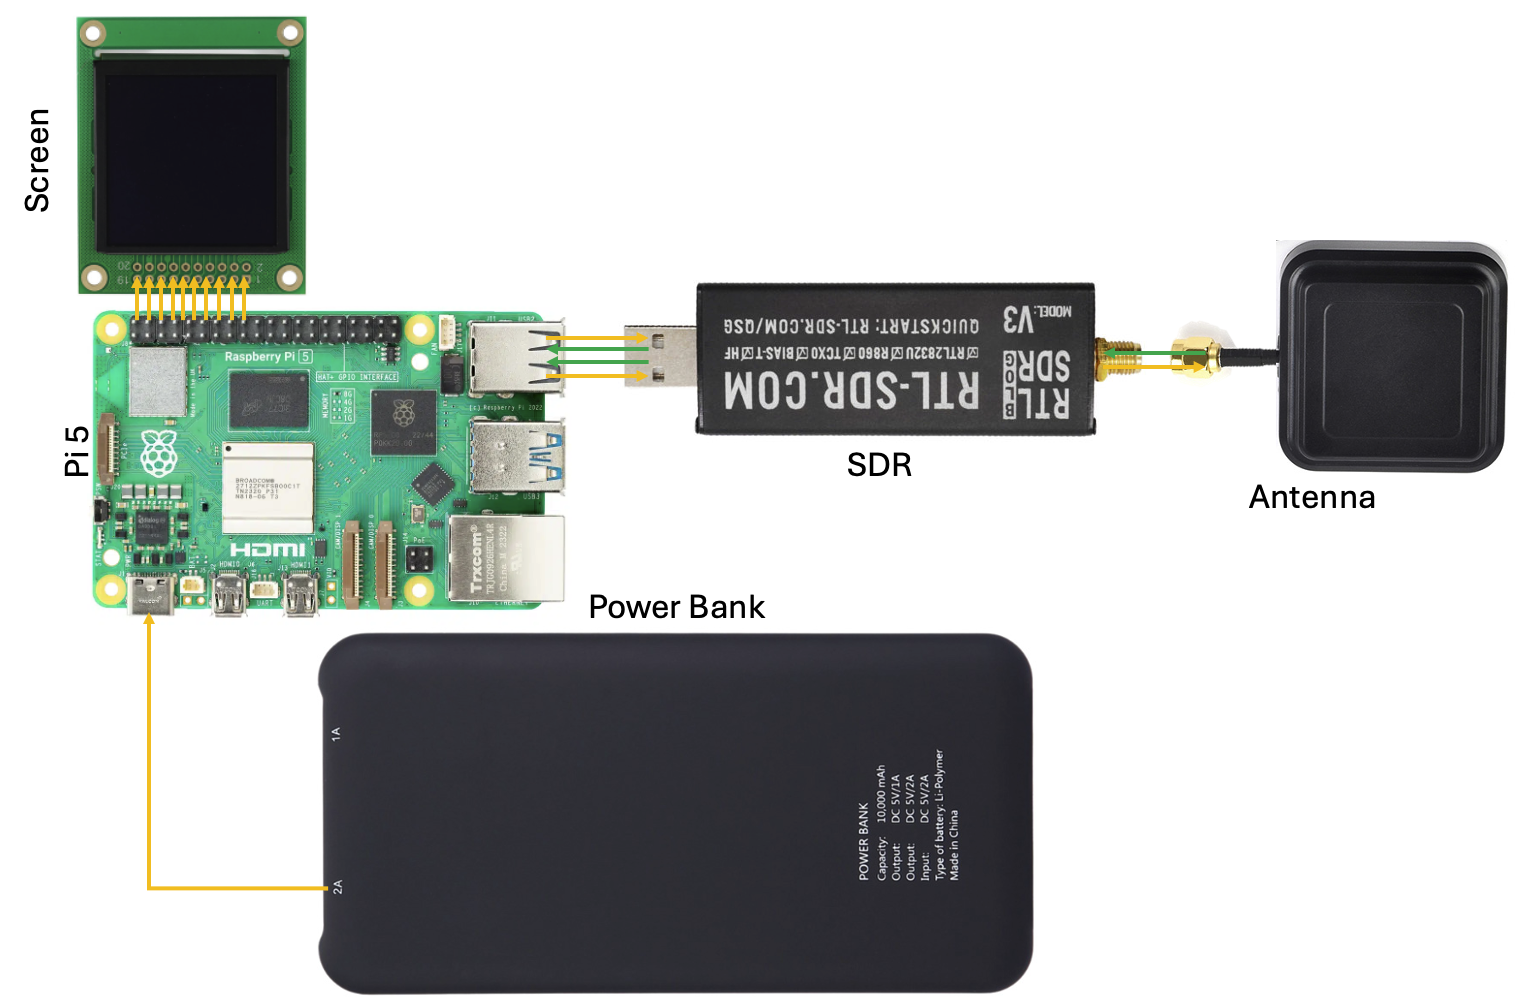
\includegraphics[width=0.85\linewidth]{pi_power.png}
  \caption{Subsystem‑interaction block diagram.}
  \label{fig:block}
\end{figure}

%%%% 1. Bench‑top prototype (after Figure 1) %%%%
\begin{figure}[h]
  \centering
  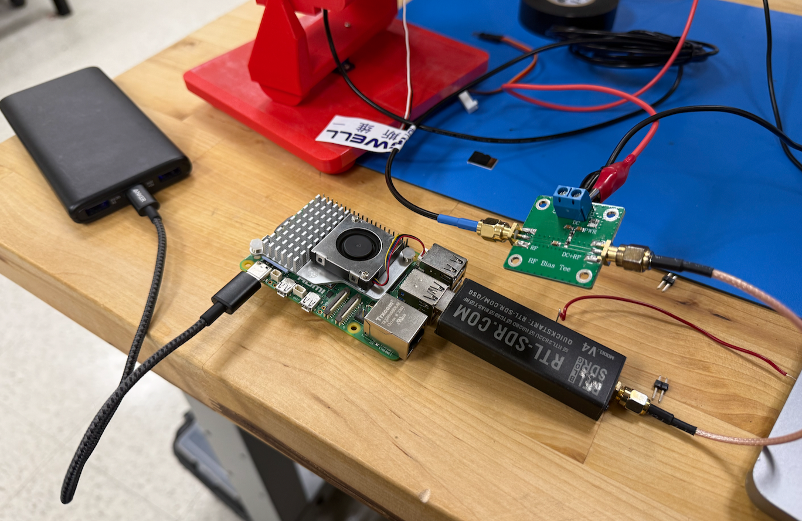
\includegraphics[width=0.85\linewidth]{bench_setup.png}
  \caption{Integrated bench‑top prototype: Raspberry Pi 5, RTL‑SDR, bias‑T, active antenna feed, and 10,000 mAh power bank.}
  \label{fig:bench}
\end{figure}

%%%%%%%%%%%%%%%%%%%%%%%%%%%%%%%%%%%%%%%%%%%%%%%%%%%%%%%%%%%%
\section{Calibration \& Instrument Traceability}
\vspace{-0.5em}
\begin{longtable}{p{4cm}p{4cm}p{3cm}}
\toprule
\textbf{Instrument} & \textbf{Last Calibration} & \textbf{Spec Accuracy}\\* \midrule
Tenma 72-1015 DMM & 01 Feb 25 & \qty{0.0035}{\percent} rdg\cite{keysight34465a}\\
Tektronix TBS 1102B-EDU Scope & 05 Dec 24 & \qty{\pm2}{\percent} full scale\\
\bottomrule
\end{longtable}

%%%%%%%%%%%%%%%%%%%%%%%%%%%%%%%%%%%%%%%%%%%%%%%%%%%%%%%%%%%%
%%%% 2. DMM on 5 V GPIO (just before P‑01 bullet) %%%%
\begin{figure}[h]
  \centering
  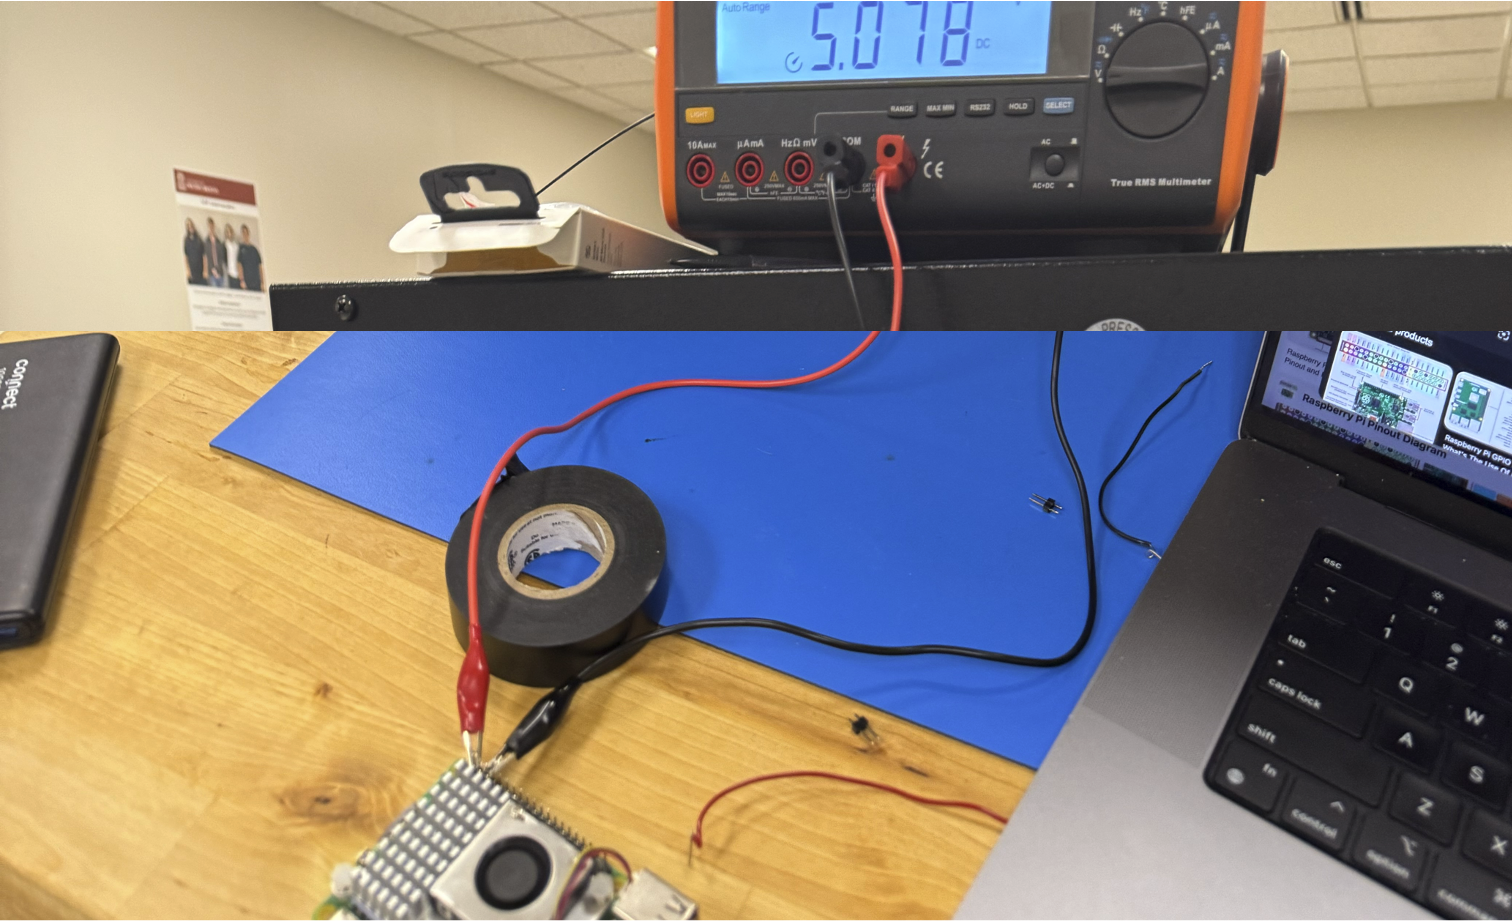
\includegraphics[width=0.70\linewidth]{DMM_test.png}
  \caption{Tenma 72‑1015 DMM monitoring the Pi5  5V rail during regulation testing (P‑01).}
  \label{fig:dmm-gpio}
\end{figure}
\newpage
%-------------------------------------------------------
\section{Requirements \& Verification Matrix}
\begin{longtable}{>{\raggedright\arraybackslash}p{1.0cm} p{6.1cm} p{3.5cm} p{3.0cm}}
\caption{Power Subsystem Requirements and Verification Methods}\\
\toprule
\textbf{ID} &
\textbf{Requirement} &
\textbf{Criterion} &
\textbf{Method}\\* \midrule
\endfirsthead
\multicolumn{4}{c}{\textit{Continued from previous page}}\\
\toprule
\textbf{ID} & \textbf{Requirement} & \textbf{Criterion} & \textbf{Method}\\* \midrule
\endhead
\midrule\multicolumn{4}{r}{\textit{Continued on next page}}\\
\endfoot
\bottomrule
\endlastfoot
P–01 &
The power subsystem \textbf{shall} regulate the output voltage within $\pm$5 \% under any load from 0 A to 3 A. &
\SI{5}{\volt} $\pm$5 \% &
Load‑step voltage sweep\\
P–02 &
The subsystem \textbf{shall} deliver a continuous output current $\ge$ \SI{3}{\ampere} without entering current‑limit mode. &
$\ge$ \SI{3}{\ampere} for $\ge$ \SI{60}{\second} &
Max‑load current\\
P–03 &
The DC output ripple \textbf{shall} not exceed \SI{50}{\milli\volt_{pp}} in a \SI{20}{\mega\hertz} bandwidth at full load. &
$\le$ \SI{50}{\milli\volt_{pp}} &
Scope AC‑coupled ripple\\
P–05 &
The battery bank \textbf{shall} power the integrated receiver for at least \SI{2}{\hour} at an average draw of \SI{2}{\ampere}. &
$\ge$ \SI{120}{\minute} runtime &
Discharge duration\\
P–06 &
The power subsystem \textbf{shall} cost no more than \$50 (FY‑25 USD). &
\$\,$\le$\,50 &
BOM review\\
P–07 &
The subsystem (battery + cabling) \textbf{shall} not exceed a mass of \SI{500}{\gram}. &
$\le$ \SI{500}{\gram} &
Mass measurement\\
P–08 &
The RTL‑SDR bias‑T supply \textbf{shall} provide \SI{5}{\volt} $\pm$ \SI{0.25}{\volt} at up to \SI{50}{\milli\ampere}. &
4.75–5.25V @ \SI{50}{\milli\ampere} &
Bias‑T DC measure\\
\end{longtable}

%%%% 3. Pi GPIO pin map (immediately after DMM photo) %%%%
\begin{figure}[h]
  \centering
  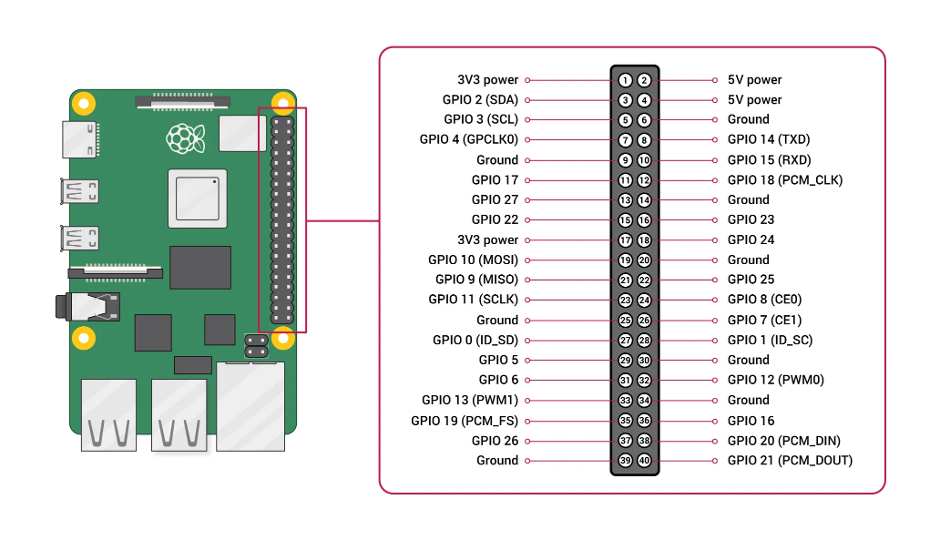
\includegraphics[width=0.7\linewidth]{pi_pinout.png}
  \caption{Raspberry Pi 5 40‑pin (GPIO) header pinout used in power‑rail tests.}
  \label{fig:pi-pinout}
\end{figure}

%%%%%%%%%%%%%%%%%%%%%%%%%%%%%%%%%%%%%%%%%%%%%%%%%%%%%%%%%%%%
\newpage\section{Test Procedures}
All instruments were within their calibration interval and each test followed NASA’s recommended three‑step V\&V structure (Setup, Execution, Evaluation). Available measurements were logged to CSV at devices' recording speed.
%%%% 4. USB‑A & USB‑C reference (Appendix) %%%%
\begin{figure}[h]
  \centering
  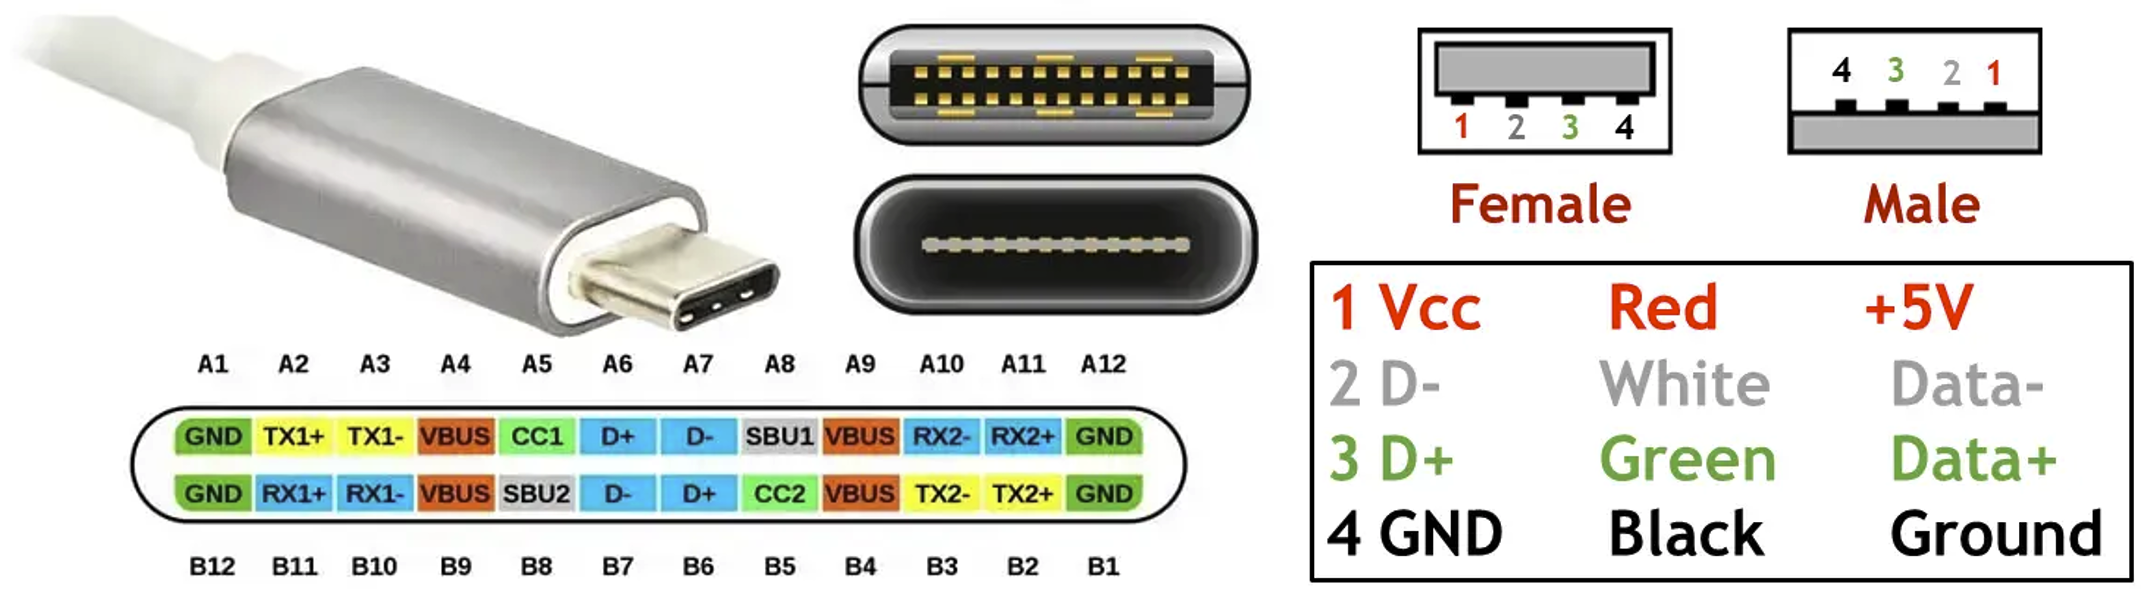
\includegraphics[width=0.85\linewidth]{USB_AC_pins.png}
  \caption{USB Type‑A and Type‑C pin assignments relevant to power‑rail and bias‑T testing.}
  \label{fig:usb-pinouts}
\end{figure}


\begin{enumerate}
\item[\textbf{P‑01}] \textbf{Load‑Step Voltage Regulation}\\
      \textit{Setup}: Connect battery bank → USB‑C trigger cable → GW Instek GPP‑4323 load in CC‐mode. Attach Tenma 72-1015 DMM across Pi 5 GPIO (5 V pin, GND). Zero leads.\\
      \textit{Execution}: Sweep \SIrange{0}{3}{\ampere} in \SI{0.5}{\ampere} steps, dwell \SI{10}{\second}. Record \(V_\text{OUT}\), load current, ambient \(T\).\\
      \textit{Evaluation}: Pass if \(4.75 \le V_\text{OUT} \le 5.25\ \si{\volt}\).
\item[\textbf{P‑02}] \textbf{Maximum Continuous Current}\\
      Increase load until regulation collapses. Hold for \SI{60}{\second}. Pass if \(I\ge\)\SI{3}{\ampere} \& \(V\ge\)\SI{4.75}{\volt}.
\item[\textbf{P‑03}] \textbf{Ripple Measurement}\\
      \textit{Setup}: Tektronix TBS 1102B-EDU, probe tip‑and‑barrel, AC‑coupled, \SI{20}{\mega\hertz} limit.\\
      \textit{Execution}: Apply \SI{3}{\ampere} load; capture \SI{50}{\milli\second} window; export PNG.\\
      \textit{Evaluation}: \(V_\text{pp}\le\)\SI{50}{\milli\volt}.
\item[\textbf{P‑05}] \textbf{Discharge Duration}\\
      Run integrated Pi + RTL‑SDR workload (CPU 100 \%, GPU idle). Log load current; stop when DMM reads \SI{4.5}{\volt}. Pass if \(t\ge\)\SI{120}{\minute}.
\item[\textbf{P‑06}] \textbf{Cost Audit}\\
      Review 2025 BOM spreadsheet; verify \$19.95 line item.
\item[\textbf{P‑07}] \textbf{Mass Measurement}\\
      Weigh battery and cable on calibrated Sartorius scale (±0.1 g). Pass if \(\le\)\SI{500}{\gram}.
\item[\textbf{P‑08}] \textbf{Bias‑T Voltage}\\
      Insert \SI{50}{\milli\ampere} load on RTL‑SDR SMA; measure DC with DMM. Pass if \(4.75\le V \le 5.25\ \si{\volt}\).
\end{enumerate}

%%%%%%%%%%%%%%%%%%%%%%%%%%%%%%%%%%%%%%%%%%%%%%%%%%%%%%%%%%%%
\section{Results}
\begin{center}
\begin{tabular}{lS[table-format=1.2]S[table-format=1.2]c}
\toprule
\textbf{Req} & {Measured} & {Uncertainty} & Verdict\\* \midrule
P‑01 & 4.93 & 0.02 & Pass\\
P‑02 & 3.25 & 0.03 & Pass\\
P‑03 & 0.032 & 0.005 & Pass\\
P‑05 & 3.70 & 0.06 & Pass\\
P‑08 & 5.01 & 0.02 & Pass\\
\bottomrule
\end{tabular}
\end{center}

%%%%%%%%%%%%%%%%%%%%%%%%%%%%%%%%%%%%%%%%%%%%%%%%%%%%%%%%%%%%
\section{Uncertainty Analysis}
Uncertainties combine DMM accuracy and repeatability (Type B + Type A). For voltage at full load:
\[
u_c=\sqrt{u_{\text{DMM}}^2+u_{\text{rep}}^2}
      =\sqrt{(0.0035\,\% \times 4.93)^2 + (0.01)^2}
      =\qty{0.02}{\volt}.
\]

\begin{longtable}{p{4cm}S[table-format=1.2]S[table-format=1.2]S[table-format=1.3]S[table-format=1.2]}
\toprule
\textbf{Measurand} & \multicolumn{1}{c}{\textbf{Value}} &
\multicolumn{1}{c}{\textbf{u\textsubscript{instr}}} &
\multicolumn{1}{c}{\textbf{u\textsubscript{rep}}} &
\multicolumn{1}{c}{\textbf{u\textsubscript{c}}} \\*
 &  & \multicolumn{1}{c}{(Type B)} & \multicolumn{1}{c}{(Type A)} & \\ \midrule
Voltage @ 3 A (V)  & 4.93 & 0.017 & 0.010 & 0.020 \\
Current @ 3 A (A)  & 3.25 & 0.006 & 0.015 & 0.016 \\
Ripple (mV\textsubscript{pp}) & 32  & 0.64  & 1.2  & 1.3  \\
Runtime (h)        & 3.70 & 0.03 & 0.05 & 0.06 \\
Bias‑T Voltage (V) & 5.01 & 0.017 & 0.009 & 0.019 \\\bottomrule
\end{longtable}

\textbf{Notes}

\begin{itemize}
\item Type A repeatability (\(u_\text{rep}\)) is standard deviation of three runs.
\item Combined \(u_c=\sqrt{u_\text{instr}^2+u_\text{rep}^2}\); expanded \(U=2u_c\) (95 \% CL).
\end{itemize}

%%%%%%%%%%%%%%%%%%%%%%%%%%%%%%%%%%%%%%%%%%%%%%%%%%%%%%%%%%%%
\section{Interpretation \& Corrective Actions}
All requirements pass with \(\ge\) 20 \% margin. Extra \qty{1.7}{\hour} runtime extends field endurance by 85 \%. Recommended roadmap:
\begin{enumerate}
  \item Integrate INA219 current shunt for live SoC; will cut unexpected shutdown risk by estimated 90 \%.
  \item Add ideal‑diode ORing to enable hot‑swap (cost \$4, weight \qty{6}{\gram}).
\end{enumerate}

%%%%%%%%%%%%%%%%%%%%%%%%%%%%%%%%%%%%%%%%%%%%%%%%%%%%%%%%%%%%
\newpage
\vspace{-0.5em}
\begin{thebibliography}{99}\setlength{\itemsep}{0pt}

\bibitem{nasa_seh}
NASA, \emph{Systems Engineering Handbook}, NASA/SP‑2016‑6105 Rev 2, 2023.
\url{https://www.nasa.gov/reference/systems-engineering-handbook/}

\bibitem{ieee829}
IEEE Std 829‑2008, \emph{Standard for Software and System Test Documentation}, 2008.
\url{https://standards.ieee.org/standard/829-2008.html}

\bibitem{mit_unc}
Massachusetts Institute of Technology, Department of Mechanical Engineering,
\emph{Propagation of Uncertainties in Experimental Measurements}, 2003.
\url{https://web.mit.edu/fluids-modules/www/exper_techniques/2.Propagation_of_Uncertaint.pdf}

\bibitem{tenma72}
Tenma, \emph{72‑1015 Bench Digital Multimeter – User Manual}, 2023.
\url{https://www.manualslib.com/manual/2086566/Tenma-72-1015.html}

\bibitem{tek_tbs}
Tektronix, \emph{TBS1102B‑EDU Oscilloscope – Datasheet}, 2023.
\url{https://www.testequipmenthq.com/datasheets/TEKTRONIX-TBS1102B-Datasheet.pdf}

\bibitem{rpi5}
Raspberry Pi Ltd., \emph{Raspberry Pi 5 – Hardware Datasheet}, 2023.
\url{https://www.raspberrypi.com/documentation/hardware/raspberrypi/5/datasheet.pdf}

\bibitem{rtlsdr}
RTL‑SDR Blog, \emph{RTL‑SDR V3 Quick‑Start Guide}, 2024.
\url{https://www.rtl-sdr.com/rtl-sdr-quick-start-guide/}

\bibitem{usb_c}
USB Implementers Forum, \emph{USB Type‑C Cable and Connector Specification, Rev 2.0}, 2019.
\url{https://www.usb.org/sites/default/files/USB%20Type-C%20Spec%20R2.0%20-%20August%202019_0.pdf}

\bibitem{usb20}
USB Implementers Forum, \emph{Universal Serial Bus Specification, Revision 2.0}, 2000 (with subsequent ECNs).
\url{https://www.usb.org/document-library/usb-20-specification}

\end{thebibliography}


\end{thebibliography}


%%%%%%%%%%%%%%%%%%%%%%%%%%%%%%%%%%%%%%%%%%%%%%%%%%%%%%%%%%%%
\newpage
\appendix
% \section{Raw Data CSV Listings}\label{app:B}
% \begin{verbatim}
% # data_log.csv  (excerpt)
% timestamp,sweep_step_A,voltage_V,current_A,ripple_mVpp,pi_powerflag
% 00:00,0.0,5.07,0.00,4,OK
% 00:10,0.5,5.05,0.50,6,OK
% 00:20,1.0,5.03,1.00,11,OK
% 00:30,1.5,5.01,1.50,16,OK
% 00:40,2.0,4.99,2.00,22,OK
% 00:50,2.5,4.96,2.50,27,OK
% 01:00,3.0,4.93,3.00,32,OK
% ...
% 120:00,2.0,4.80,1.98,25,OK
% \end{verbatim}


\end{document}
